\documentclass[twoside]{book}

% Packages required by doxygen
\usepackage{fixltx2e}
\usepackage{calc}
\usepackage{doxygen}
\usepackage[export]{adjustbox} % also loads graphicx
\usepackage{graphicx}
\usepackage[utf8]{inputenc}
\usepackage{makeidx}
\usepackage{multicol}
\usepackage{multirow}
\PassOptionsToPackage{warn}{textcomp}
\usepackage{textcomp}
\usepackage[nointegrals]{wasysym}
\usepackage[table]{xcolor}

% Font selection
\usepackage[T1]{fontenc}
\usepackage[scaled=.90]{helvet}
\usepackage{courier}
\usepackage{amssymb}
\usepackage{sectsty}
\renewcommand{\familydefault}{\sfdefault}
\allsectionsfont{%
  \fontseries{bc}\selectfont%
  \color{darkgray}%
}
\renewcommand{\DoxyLabelFont}{%
  \fontseries{bc}\selectfont%
  \color{darkgray}%
}
\newcommand{\+}{\discretionary{\mbox{\scriptsize$\hookleftarrow$}}{}{}}

% Page & text layout
\usepackage{geometry}
\geometry{%
  a4paper,%
  top=2.5cm,%
  bottom=2.5cm,%
  left=2.5cm,%
  right=2.5cm%
}
\tolerance=750
\hfuzz=15pt
\hbadness=750
\setlength{\emergencystretch}{15pt}
\setlength{\parindent}{0cm}
\setlength{\parskip}{3ex plus 2ex minus 2ex}
\makeatletter
\renewcommand{\paragraph}{%
  \@startsection{paragraph}{4}{0ex}{-1.0ex}{1.0ex}{%
    \normalfont\normalsize\bfseries\SS@parafont%
  }%
}
\renewcommand{\subparagraph}{%
  \@startsection{subparagraph}{5}{0ex}{-1.0ex}{1.0ex}{%
    \normalfont\normalsize\bfseries\SS@subparafont%
  }%
}
\makeatother

% Headers & footers
\usepackage{fancyhdr}
\pagestyle{fancyplain}
\fancyhead[LE]{\fancyplain{}{\bfseries\thepage}}
\fancyhead[CE]{\fancyplain{}{}}
\fancyhead[RE]{\fancyplain{}{\bfseries\leftmark}}
\fancyhead[LO]{\fancyplain{}{\bfseries\rightmark}}
\fancyhead[CO]{\fancyplain{}{}}
\fancyhead[RO]{\fancyplain{}{\bfseries\thepage}}
\fancyfoot[LE]{\fancyplain{}{}}
\fancyfoot[CE]{\fancyplain{}{}}
\fancyfoot[RE]{\fancyplain{}{\bfseries\scriptsize Generated by Doxygen }}
\fancyfoot[LO]{\fancyplain{}{\bfseries\scriptsize Generated by Doxygen }}
\fancyfoot[CO]{\fancyplain{}{}}
\fancyfoot[RO]{\fancyplain{}{}}
\renewcommand{\footrulewidth}{0.4pt}
\renewcommand{\chaptermark}[1]{%
  \markboth{#1}{}%
}
\renewcommand{\sectionmark}[1]{%
  \markright{\thesection\ #1}%
}

% Indices & bibliography
\usepackage{natbib}
\usepackage[titles]{tocloft}
\setcounter{tocdepth}{3}
\setcounter{secnumdepth}{5}
\makeindex

% Hyperlinks (required, but should be loaded last)
\usepackage{ifpdf}
\ifpdf
  \usepackage[pdftex,pagebackref=true]{hyperref}
\else
  \usepackage[ps2pdf,pagebackref=true]{hyperref}
\fi
\hypersetup{%
  colorlinks=true,%
  linkcolor=blue,%
  citecolor=blue,%
  unicode%
}

% Custom commands
\newcommand{\clearemptydoublepage}{%
  \newpage{\pagestyle{empty}\cleardoublepage}%
}

\usepackage{caption}
\captionsetup{labelsep=space,justification=centering,font={bf},singlelinecheck=off,skip=4pt,position=top}

%===== C O N T E N T S =====

\begin{document}

% Titlepage & ToC
\hypersetup{pageanchor=false,
             bookmarksnumbered=true,
             pdfencoding=unicode
            }
\pagenumbering{roman}
\begin{titlepage}
\vspace*{7cm}
\begin{center}%
{\Large Lane Detection for Autonomous Cars }\\
\vspace*{1cm}
{\large Generated by Doxygen 1.8.11}\\
\end{center}
\end{titlepage}
\clearemptydoublepage
\tableofcontents
\clearemptydoublepage
\pagenumbering{arabic}
\hypersetup{pageanchor=true}

%--- Begin generated contents ---
\chapter{Class Index}
\section{Class List}
Here are the classes, structs, unions and interfaces with brief descriptions\+:\begin{DoxyCompactList}
\item\contentsline{section}{\hyperlink{classLaneDetector}{Lane\+Detector} \\*Definition of the \hyperlink{classLaneDetector}{Lane\+Detector} class. It contains all the functions and variables depicted in the }{\pageref{classLaneDetector}}{}
\end{DoxyCompactList}

\chapter{File Index}
\section{File List}
Here is a list of all documented files with brief descriptions\+:\begin{DoxyCompactList}
\item\contentsline{section}{/home/michi/\+Desktop/\+U\+M\+D/\+E\+N\+P\+M808\+X/\+Midterm/workspace/\+Lane-\/\+Detection-\/for-\/\+Autonomous-\/\+Cars/include/\hyperlink{LaneDetector_8hpp}{Lane\+Detector.\+hpp} \\*Header file for the \hyperlink{classLaneDetector}{Lane\+Detector} class. Functions are developed in \hyperlink{LaneDetector_8cpp}{Lane\+Detector.\+cpp} }{\pageref{LaneDetector_8hpp}}{}
\item\contentsline{section}{/home/michi/\+Desktop/\+U\+M\+D/\+E\+N\+P\+M808\+X/\+Midterm/workspace/\+Lane-\/\+Detection-\/for-\/\+Autonomous-\/\+Cars/\+Lane\+Detector/\hyperlink{demo_8cpp}{demo.\+cpp} \\*Demo code that shows the full functionality of the \hyperlink{classLaneDetector}{Lane\+Detector} object }{\pageref{demo_8cpp}}{}
\item\contentsline{section}{/home/michi/\+Desktop/\+U\+M\+D/\+E\+N\+P\+M808\+X/\+Midterm/workspace/\+Lane-\/\+Detection-\/for-\/\+Autonomous-\/\+Cars/\+Lane\+Detector/\hyperlink{LaneDetector_8cpp}{Lane\+Detector.\+cpp} \\*Definition of all the function that form part of the \hyperlink{classLaneDetector}{Lane\+Detector} class }{\pageref{LaneDetector_8cpp}}{}
\item\contentsline{section}{/home/michi/\+Desktop/\+U\+M\+D/\+E\+N\+P\+M808\+X/\+Midterm/workspace/\+Lane-\/\+Detection-\/for-\/\+Autonomous-\/\+Cars/test/\hyperlink{main_8cpp}{main.\+cpp} \\*Test cases for code coverage }{\pageref{main_8cpp}}{}
\item\contentsline{section}{/home/michi/\+Desktop/\+U\+M\+D/\+E\+N\+P\+M808\+X/\+Midterm/workspace/\+Lane-\/\+Detection-\/for-\/\+Autonomous-\/\+Cars/test/\hyperlink{test_8cpp}{test.\+cpp} \\*Test cases for code coverage }{\pageref{test_8cpp}}{}
\end{DoxyCompactList}

\chapter{Class Documentation}
\hypertarget{classLaneDetector}{}\section{Lane\+Detector Class Reference}
\label{classLaneDetector}\index{Lane\+Detector@{Lane\+Detector}}


Definition of the \hyperlink{classLaneDetector}{Lane\+Detector} class. It contains all the functions and variables depicted in the.  




{\ttfamily \#include $<$Lane\+Detector.\+hpp$>$}

\subsection*{Public Member Functions}
\begin{DoxyCompactItemize}
\item 
cv\+::\+Mat \hyperlink{classLaneDetector_a816d7555c6b7690d7afdd81eb62dd35b}{de\+Noise} (cv\+::\+Mat input\+Image)
\begin{DoxyCompactList}\small\item\em Apply gaussian filter to the input image to denoise it. \end{DoxyCompactList}\item 
cv\+::\+Mat \hyperlink{classLaneDetector_a8920b291267aad638f8874512fba33cf}{edge\+Detector} (cv\+::\+Mat img\+\_\+noise)
\begin{DoxyCompactList}\small\item\em Detect all the edges in the blurred frame by filtering the image. \end{DoxyCompactList}\item 
cv\+::\+Mat \hyperlink{classLaneDetector_a64d74d2971d1e14175ef58dfbb391f6d}{mask} (cv\+::\+Mat img\+\_\+edges)
\begin{DoxyCompactList}\small\item\em Mask the image so that only the edges that form part of the lane are detected. \end{DoxyCompactList}\item 
std\+::vector$<$ cv\+::\+Vec4i $>$ \hyperlink{classLaneDetector_adbbc2f50aee10844aeec12b1fe084fb2}{hough\+Lines} (cv\+::\+Mat img\+\_\+mask)
\begin{DoxyCompactList}\small\item\em Obtain all the line segments in the masked images which are going to be part of the lane boundaries. \end{DoxyCompactList}\item 
std\+::vector$<$ std\+::vector$<$ cv\+::\+Vec4i $>$ $>$ \hyperlink{classLaneDetector_a8005c489f194eded3bc5a76cfc496c43}{line\+Separation} (std\+::vector$<$ cv\+::\+Vec4i $>$ lines, cv\+::\+Mat img\+\_\+edges)
\begin{DoxyCompactList}\small\item\em Sort all the detected Hough lines by slope. \end{DoxyCompactList}\item 
std\+::vector$<$ cv\+::\+Point $>$ \hyperlink{classLaneDetector_ac9a862f41a23ab0c3bfed2ce512a56d8}{regression} (std\+::vector$<$ std\+::vector$<$ cv\+::\+Vec4i $>$ $>$ left\+\_\+right\+\_\+lines, cv\+::\+Mat input\+Image)
\begin{DoxyCompactList}\small\item\em Regression takes all the classified line segments initial and final points and fits a new lines out of them using the method of least squares. \end{DoxyCompactList}\item 
std\+::string \hyperlink{classLaneDetector_a84053373ae184e752f023658fb187241}{predict\+Turn} ()
\begin{DoxyCompactList}\small\item\em Predict if the lane is turning left, right or if it is going straight. \end{DoxyCompactList}\item 
int \hyperlink{classLaneDetector_a9564c3349f0fa5a7da7968b9461e2730}{plot\+Lane} (cv\+::\+Mat input\+Image, std\+::vector$<$ cv\+::\+Point $>$, std\+::string turn)
\begin{DoxyCompactList}\small\item\em This function plots both sides of the lane, the turn prediction message and a transparent polygon that covers the area inside the lane boundaries. \end{DoxyCompactList}\end{DoxyCompactItemize}


\subsection{Detailed Description}
Definition of the \hyperlink{classLaneDetector}{Lane\+Detector} class. It contains all the functions and variables depicted in the. 

Activity diagram and U\+ML Class diagram. It detects the lanes in an image if a highway and outputs the same image with the plotted lane. 

\subsection{Member Function Documentation}
\index{Lane\+Detector@{Lane\+Detector}!de\+Noise@{de\+Noise}}
\index{de\+Noise@{de\+Noise}!Lane\+Detector@{Lane\+Detector}}
\subsubsection[{\texorpdfstring{de\+Noise(cv\+::\+Mat input\+Image)}{deNoise(cv::Mat inputImage)}}]{\setlength{\rightskip}{0pt plus 5cm}cv\+::\+Mat Lane\+Detector\+::de\+Noise (
\begin{DoxyParamCaption}
\item[{cv\+::\+Mat}]{input\+Image}
\end{DoxyParamCaption}
)}\hypertarget{classLaneDetector_a816d7555c6b7690d7afdd81eb62dd35b}{}\label{classLaneDetector_a816d7555c6b7690d7afdd81eb62dd35b}


Apply gaussian filter to the input image to denoise it. 


\begin{DoxyParams}{Parameters}
{\em input\+Image} & is the frame of a video in which the \\
\hline
{\em lane} & is going to be detected \\
\hline
\end{DoxyParams}
\begin{DoxyReturn}{Returns}
Blurred and denoised image 
\end{DoxyReturn}
\index{Lane\+Detector@{Lane\+Detector}!edge\+Detector@{edge\+Detector}}
\index{edge\+Detector@{edge\+Detector}!Lane\+Detector@{Lane\+Detector}}
\subsubsection[{\texorpdfstring{edge\+Detector(cv\+::\+Mat img\+\_\+noise)}{edgeDetector(cv::Mat img_noise)}}]{\setlength{\rightskip}{0pt plus 5cm}cv\+::\+Mat Lane\+Detector\+::edge\+Detector (
\begin{DoxyParamCaption}
\item[{cv\+::\+Mat}]{img\+\_\+noise}
\end{DoxyParamCaption}
)}\hypertarget{classLaneDetector_a8920b291267aad638f8874512fba33cf}{}\label{classLaneDetector_a8920b291267aad638f8874512fba33cf}


Detect all the edges in the blurred frame by filtering the image. 


\begin{DoxyParams}{Parameters}
{\em img\+\_\+noise} & is the previously blurred frame \\
\hline
\end{DoxyParams}
\begin{DoxyReturn}{Returns}
Binary image with only the edges represented in white 
\end{DoxyReturn}
\index{Lane\+Detector@{Lane\+Detector}!hough\+Lines@{hough\+Lines}}
\index{hough\+Lines@{hough\+Lines}!Lane\+Detector@{Lane\+Detector}}
\subsubsection[{\texorpdfstring{hough\+Lines(cv\+::\+Mat img\+\_\+mask)}{houghLines(cv::Mat img_mask)}}]{\setlength{\rightskip}{0pt plus 5cm}std\+::vector$<$ cv\+::\+Vec4i $>$ Lane\+Detector\+::hough\+Lines (
\begin{DoxyParamCaption}
\item[{cv\+::\+Mat}]{img\+\_\+mask}
\end{DoxyParamCaption}
)}\hypertarget{classLaneDetector_adbbc2f50aee10844aeec12b1fe084fb2}{}\label{classLaneDetector_adbbc2f50aee10844aeec12b1fe084fb2}


Obtain all the line segments in the masked images which are going to be part of the lane boundaries. 


\begin{DoxyParams}{Parameters}
{\em img\+\_\+mask} & is the masked binary image from the previous function \\
\hline
\end{DoxyParams}
\begin{DoxyReturn}{Returns}
Vector that contains all the detected lines in the image 
\end{DoxyReturn}
\index{Lane\+Detector@{Lane\+Detector}!line\+Separation@{line\+Separation}}
\index{line\+Separation@{line\+Separation}!Lane\+Detector@{Lane\+Detector}}
\subsubsection[{\texorpdfstring{line\+Separation(std\+::vector$<$ cv\+::\+Vec4i $>$ lines, cv\+::\+Mat img\+\_\+edges)}{lineSeparation(std::vector< cv::Vec4i > lines, cv::Mat img_edges)}}]{\setlength{\rightskip}{0pt plus 5cm}std\+::vector$<$ std\+::vector$<$ cv\+::\+Vec4i $>$ $>$ Lane\+Detector\+::line\+Separation (
\begin{DoxyParamCaption}
\item[{std\+::vector$<$ cv\+::\+Vec4i $>$}]{lines, }
\item[{cv\+::\+Mat}]{img\+\_\+edges}
\end{DoxyParamCaption}
)}\hypertarget{classLaneDetector_a8005c489f194eded3bc5a76cfc496c43}{}\label{classLaneDetector_a8005c489f194eded3bc5a76cfc496c43}


Sort all the detected Hough lines by slope. 

The lines are classified into right or left depending on the sign of their slope and their approximate location 
\begin{DoxyParams}{Parameters}
{\em lines} & is the vector that contains all the detected lines \\
\hline
{\em img\+\_\+edges} & is used for determining the image center \\
\hline
\end{DoxyParams}
\begin{DoxyReturn}{Returns}
The output is a vector(2) that contains all the classified lines 
\end{DoxyReturn}
\index{Lane\+Detector@{Lane\+Detector}!mask@{mask}}
\index{mask@{mask}!Lane\+Detector@{Lane\+Detector}}
\subsubsection[{\texorpdfstring{mask(cv\+::\+Mat img\+\_\+edges)}{mask(cv::Mat img_edges)}}]{\setlength{\rightskip}{0pt plus 5cm}cv\+::\+Mat Lane\+Detector\+::mask (
\begin{DoxyParamCaption}
\item[{cv\+::\+Mat}]{img\+\_\+edges}
\end{DoxyParamCaption}
)}\hypertarget{classLaneDetector_a64d74d2971d1e14175ef58dfbb391f6d}{}\label{classLaneDetector_a64d74d2971d1e14175ef58dfbb391f6d}


Mask the image so that only the edges that form part of the lane are detected. 


\begin{DoxyParams}{Parameters}
{\em img\+\_\+edges} & is the edges image from the previous function \\
\hline
\end{DoxyParams}
\begin{DoxyReturn}{Returns}
Binary image with only the desired edges being represented 
\end{DoxyReturn}
\index{Lane\+Detector@{Lane\+Detector}!plot\+Lane@{plot\+Lane}}
\index{plot\+Lane@{plot\+Lane}!Lane\+Detector@{Lane\+Detector}}
\subsubsection[{\texorpdfstring{plot\+Lane(cv\+::\+Mat input\+Image, std\+::vector$<$ cv\+::\+Point $>$, std\+::string turn)}{plotLane(cv::Mat inputImage, std::vector< cv::Point >, std::string turn)}}]{\setlength{\rightskip}{0pt plus 5cm}int Lane\+Detector\+::plot\+Lane (
\begin{DoxyParamCaption}
\item[{cv\+::\+Mat}]{input\+Image, }
\item[{std\+::vector$<$ cv\+::\+Point $>$}]{lane, }
\item[{std\+::string}]{turn}
\end{DoxyParamCaption}
)}\hypertarget{classLaneDetector_a9564c3349f0fa5a7da7968b9461e2730}{}\label{classLaneDetector_a9564c3349f0fa5a7da7968b9461e2730}


This function plots both sides of the lane, the turn prediction message and a transparent polygon that covers the area inside the lane boundaries. 


\begin{DoxyParams}{Parameters}
{\em input\+Image} & is the original captured frame \\
\hline
{\em lane} & is the vector containing the information of both lines \\
\hline
{\em turn} & is the output string containing the turn information \\
\hline
\end{DoxyParams}
\begin{DoxyReturn}{Returns}
The function returns a 0 
\end{DoxyReturn}
\index{Lane\+Detector@{Lane\+Detector}!predict\+Turn@{predict\+Turn}}
\index{predict\+Turn@{predict\+Turn}!Lane\+Detector@{Lane\+Detector}}
\subsubsection[{\texorpdfstring{predict\+Turn()}{predictTurn()}}]{\setlength{\rightskip}{0pt plus 5cm}std\+::string Lane\+Detector\+::predict\+Turn (
\begin{DoxyParamCaption}
{}
\end{DoxyParamCaption}
)}\hypertarget{classLaneDetector_a84053373ae184e752f023658fb187241}{}\label{classLaneDetector_a84053373ae184e752f023658fb187241}


Predict if the lane is turning left, right or if it is going straight. 

It is done by seeing where the vanishing point is with respect to the center of the image \begin{DoxyReturn}{Returns}
String that says if there is left or right turn or if the road is straight 
\end{DoxyReturn}
\index{Lane\+Detector@{Lane\+Detector}!regression@{regression}}
\index{regression@{regression}!Lane\+Detector@{Lane\+Detector}}
\subsubsection[{\texorpdfstring{regression(std\+::vector$<$ std\+::vector$<$ cv\+::\+Vec4i $>$ $>$ left\+\_\+right\+\_\+lines, cv\+::\+Mat input\+Image)}{regression(std::vector< std::vector< cv::Vec4i > > left_right_lines, cv::Mat inputImage)}}]{\setlength{\rightskip}{0pt plus 5cm}std\+::vector$<$ cv\+::\+Point $>$ Lane\+Detector\+::regression (
\begin{DoxyParamCaption}
\item[{std\+::vector$<$ std\+::vector$<$ cv\+::\+Vec4i $>$ $>$}]{left\+\_\+right\+\_\+lines, }
\item[{cv\+::\+Mat}]{input\+Image}
\end{DoxyParamCaption}
)}\hypertarget{classLaneDetector_ac9a862f41a23ab0c3bfed2ce512a56d8}{}\label{classLaneDetector_ac9a862f41a23ab0c3bfed2ce512a56d8}


Regression takes all the classified line segments initial and final points and fits a new lines out of them using the method of least squares. 

This is done for both sides, left and right. 
\begin{DoxyParams}{Parameters}
{\em left\+\_\+right\+\_\+lines} & is the output of the line\+Separation function \\
\hline
{\em input\+Image} & is used to select where do the lines will end \\
\hline
\end{DoxyParams}
\begin{DoxyReturn}{Returns}
output contains the initial and final points of both lane boundary lines 
\end{DoxyReturn}


The documentation for this class was generated from the following files\+:\begin{DoxyCompactItemize}
\item 
/home/michi/\+Desktop/\+U\+M\+D/\+E\+N\+P\+M808\+X/\+Midterm/workspace/\+Lane-\/\+Detection-\/for-\/\+Autonomous-\/\+Cars/include/\hyperlink{LaneDetector_8hpp}{Lane\+Detector.\+hpp}\item 
/home/michi/\+Desktop/\+U\+M\+D/\+E\+N\+P\+M808\+X/\+Midterm/workspace/\+Lane-\/\+Detection-\/for-\/\+Autonomous-\/\+Cars/\+Lane\+Detector/\hyperlink{LaneDetector_8cpp}{Lane\+Detector.\+cpp}\end{DoxyCompactItemize}

\chapter{File Documentation}
\hypertarget{LaneDetector_8hpp}{}\section{/home/michi/\+Desktop/\+U\+M\+D/\+E\+N\+P\+M808\+X/\+Midterm/workspace/\+Lane-\/\+Detection-\/for-\/\+Autonomous-\/\+Cars/include/\+Lane\+Detector.hpp File Reference}
\label{LaneDetector_8hpp}\index{/home/michi/\+Desktop/\+U\+M\+D/\+E\+N\+P\+M808\+X/\+Midterm/workspace/\+Lane-\/\+Detection-\/for-\/\+Autonomous-\/\+Cars/include/\+Lane\+Detector.\+hpp@{/home/michi/\+Desktop/\+U\+M\+D/\+E\+N\+P\+M808\+X/\+Midterm/workspace/\+Lane-\/\+Detection-\/for-\/\+Autonomous-\/\+Cars/include/\+Lane\+Detector.\+hpp}}


Header file for the \hyperlink{classLaneDetector}{Lane\+Detector} class. Functions are developed in \hyperlink{LaneDetector_8cpp}{Lane\+Detector.\+cpp}.  


{\ttfamily \#include $<$opencv2/highgui/highgui.\+hpp$>$}\\*
{\ttfamily \#include $<$iostream$>$}\\*
{\ttfamily \#include $<$string$>$}\\*
{\ttfamily \#include $<$vector$>$}\\*
{\ttfamily \#include \char`\"{}opencv2/opencv.\+hpp\char`\"{}}\\*
Include dependency graph for Lane\+Detector.\+hpp\+:
\nopagebreak
\begin{figure}[H]
\begin{center}
\leavevmode
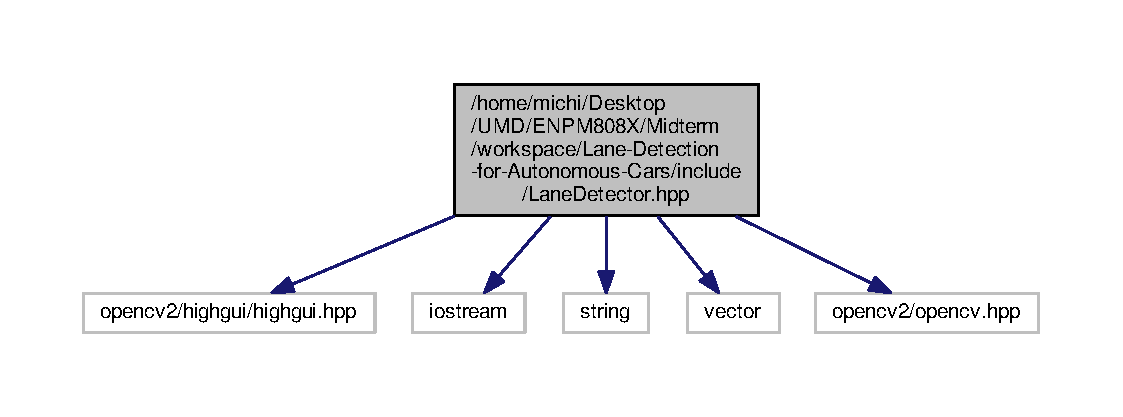
\includegraphics[width=350pt]{LaneDetector_8hpp__incl}
\end{center}
\end{figure}
This graph shows which files directly or indirectly include this file\+:
\nopagebreak
\begin{figure}[H]
\begin{center}
\leavevmode
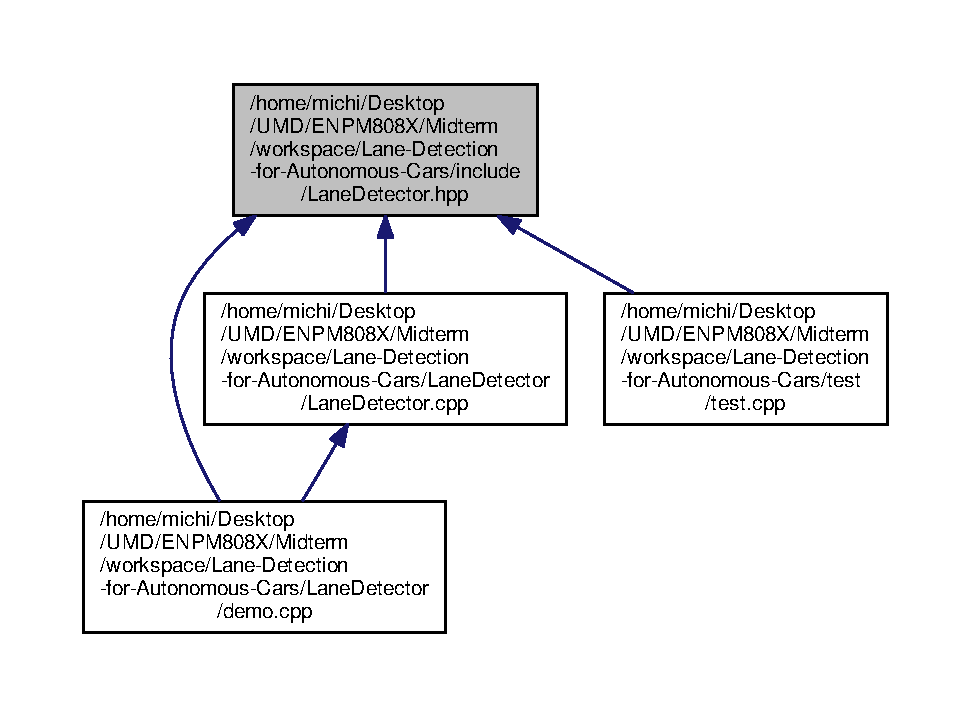
\includegraphics[width=350pt]{LaneDetector_8hpp__dep__incl}
\end{center}
\end{figure}
\subsection*{Classes}
\begin{DoxyCompactItemize}
\item 
class \hyperlink{classLaneDetector}{Lane\+Detector}
\begin{DoxyCompactList}\small\item\em Definition of the \hyperlink{classLaneDetector}{Lane\+Detector} class. It contains all the functions and variables depicted in the. \end{DoxyCompactList}\end{DoxyCompactItemize}


\subsection{Detailed Description}
Header file for the \hyperlink{classLaneDetector}{Lane\+Detector} class. Functions are developed in \hyperlink{LaneDetector_8cpp}{Lane\+Detector.\+cpp}. 

M\+IT License Copyright (c) 2017 Miguel Maestre Trueba Permission is hereby granted, free of charge, to any person obtaining a copy of this software and associated documentation files (the \char`\"{}\+Software\char`\"{}), to deal in the Software without restriction, including without limitation the rights to use, copy, modify, merge, publish, distribute, sublicense, and/or sell copies of the Software, and to permit persons to whom the Software is furnished to do so, subject to the following conditions\+: The above copyright notice and this permission notice shall be included in all copies or substantial portions of the Software. T\+HE S\+O\+F\+T\+W\+A\+RE IS P\+R\+O\+V\+I\+D\+ED \char`\"{}\+A\+S I\+S\char`\"{}, W\+I\+T\+H\+O\+UT W\+A\+R\+R\+A\+N\+TY OF A\+NY K\+I\+ND, E\+X\+P\+R\+E\+SS OR I\+M\+P\+L\+I\+ED, I\+N\+C\+L\+U\+D\+I\+NG B\+UT N\+OT L\+I\+M\+I\+T\+ED TO T\+HE W\+A\+R\+R\+A\+N\+T\+I\+ES OF M\+E\+R\+C\+H\+A\+N\+T\+A\+B\+I\+L\+I\+TY, F\+I\+T\+N\+E\+SS F\+OR A P\+A\+R\+T\+I\+C\+U\+L\+AR P\+U\+R\+P\+O\+SE A\+ND N\+O\+N\+I\+N\+F\+R\+I\+N\+G\+E\+M\+E\+NT. IN NO E\+V\+E\+NT S\+H\+A\+LL T\+HE A\+U\+T\+H\+O\+RS OR C\+O\+P\+Y\+R\+I\+G\+HT H\+O\+L\+D\+E\+RS BE L\+I\+A\+B\+LE F\+OR A\+NY C\+L\+A\+IM, D\+A\+M\+A\+G\+ES OR O\+T\+H\+ER L\+I\+A\+B\+I\+L\+I\+TY, W\+H\+E\+T\+H\+ER IN AN A\+C\+T\+I\+ON OF C\+O\+N\+T\+R\+A\+CT, T\+O\+RT OR O\+T\+H\+E\+R\+W\+I\+SE, A\+R\+I\+S\+I\+NG F\+R\+OM, O\+UT OF OR IN C\+O\+N\+N\+E\+C\+T\+I\+ON W\+I\+TH T\+HE S\+O\+F\+T\+W\+A\+RE OR T\+HE U\+SE OR O\+T\+H\+ER D\+E\+A\+L\+I\+N\+GS IN T\+HE S\+O\+F\+T\+W\+A\+RE.

\begin{DoxyCopyright}{Copyright}
Copyright 2017 Miguel Maestre Trueba
\end{DoxyCopyright}
\begin{DoxyAuthor}{Author}
Miguel Maestre Trueba 
\end{DoxyAuthor}

\hypertarget{demo_8cpp}{}\section{/home/michi/\+Desktop/\+U\+M\+D/\+E\+N\+P\+M808\+X/\+Midterm/workspace/\+Lane-\/\+Detection-\/for-\/\+Autonomous-\/\+Cars/\+Lane\+Detector/demo.cpp File Reference}
\label{demo_8cpp}\index{/home/michi/\+Desktop/\+U\+M\+D/\+E\+N\+P\+M808\+X/\+Midterm/workspace/\+Lane-\/\+Detection-\/for-\/\+Autonomous-\/\+Cars/\+Lane\+Detector/demo.\+cpp@{/home/michi/\+Desktop/\+U\+M\+D/\+E\+N\+P\+M808\+X/\+Midterm/workspace/\+Lane-\/\+Detection-\/for-\/\+Autonomous-\/\+Cars/\+Lane\+Detector/demo.\+cpp}}


Demo code that shows the full functionality of the \hyperlink{classLaneDetector}{Lane\+Detector} object.  


{\ttfamily \#include $<$opencv2/highgui/highgui.\+hpp$>$}\\*
{\ttfamily \#include $<$iostream$>$}\\*
{\ttfamily \#include $<$string$>$}\\*
{\ttfamily \#include $<$vector$>$}\\*
{\ttfamily \#include \char`\"{}opencv2/opencv.\+hpp\char`\"{}}\\*
{\ttfamily \#include \char`\"{}../include/\+Lane\+Detector.\+hpp\char`\"{}}\\*
{\ttfamily \#include \char`\"{}../\+Lane\+Detector/\+Lane\+Detector.\+cpp\char`\"{}}\\*
Include dependency graph for demo.\+cpp\+:
\nopagebreak
\begin{figure}[H]
\begin{center}
\leavevmode
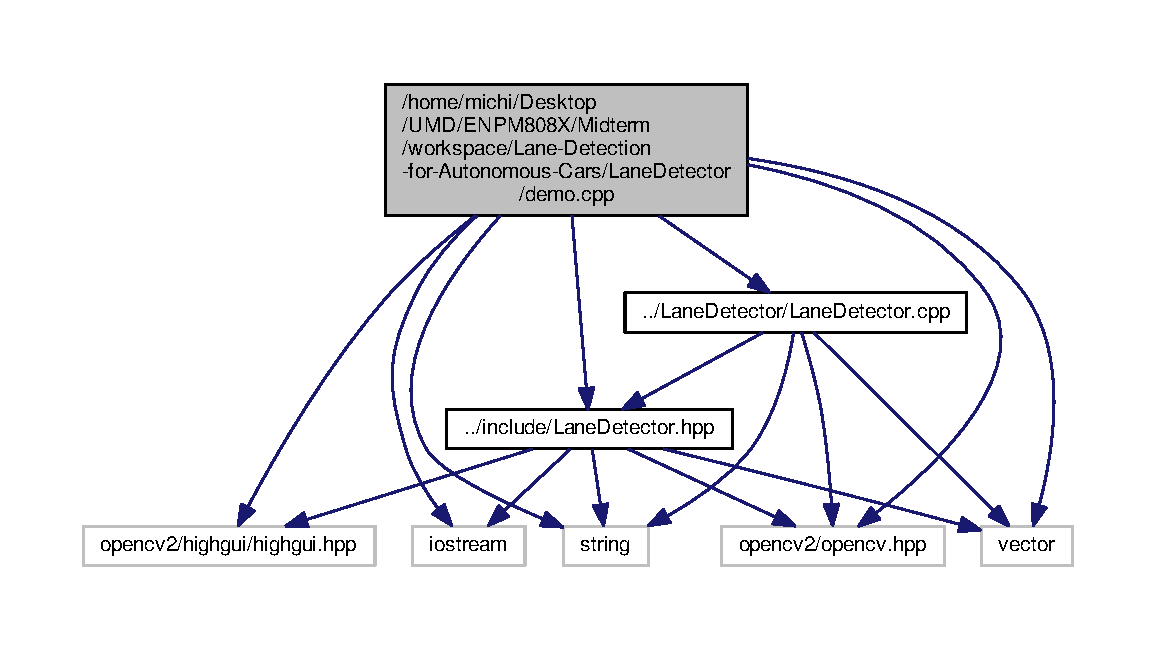
\includegraphics[width=350pt]{demo_8cpp__incl}
\end{center}
\end{figure}
\subsection*{Functions}
\begin{DoxyCompactItemize}
\item 
int \hyperlink{demo_8cpp_a0ddf1224851353fc92bfbff6f499fa97}{main} (int argc, char $\ast$argv\mbox{[}$\,$\mbox{]})
\begin{DoxyCompactList}\small\item\em Function main that runs the main algorithm of the lane detection. \end{DoxyCompactList}\end{DoxyCompactItemize}


\subsection{Detailed Description}
Demo code that shows the full functionality of the \hyperlink{classLaneDetector}{Lane\+Detector} object. 

M\+IT License Copyright (c) 2017 Miguel Maestre Trueba Permission is hereby granted, free of charge, to any person obtaining a copy of this software and associated documentation files (the \char`\"{}\+Software\char`\"{}), to deal in the Software without restriction, including without limitation the rights to use, copy, modify, merge, publish, distribute, sublicense, and/or sell copies of the Software, and to permit persons to whom the Software is furnished to do so, subject to the following conditions\+: The above copyright notice and this permission notice shall be included in all copies or substantial portions of the Software. T\+HE S\+O\+F\+T\+W\+A\+RE IS P\+R\+O\+V\+I\+D\+ED \char`\"{}\+A\+S I\+S\char`\"{}, W\+I\+T\+H\+O\+UT W\+A\+R\+R\+A\+N\+TY OF A\+NY K\+I\+ND, E\+X\+P\+R\+E\+SS OR I\+M\+P\+L\+I\+ED, I\+N\+C\+L\+U\+D\+I\+NG B\+UT N\+OT L\+I\+M\+I\+T\+ED TO T\+HE W\+A\+R\+R\+A\+N\+T\+I\+ES OF M\+E\+R\+C\+H\+A\+N\+T\+A\+B\+I\+L\+I\+TY, F\+I\+T\+N\+E\+SS F\+OR A P\+A\+R\+T\+I\+C\+U\+L\+AR P\+U\+R\+P\+O\+SE A\+ND N\+O\+N\+I\+N\+F\+R\+I\+N\+G\+E\+M\+E\+NT. IN NO E\+V\+E\+NT S\+H\+A\+LL T\+HE A\+U\+T\+H\+O\+RS OR C\+O\+P\+Y\+R\+I\+G\+HT H\+O\+L\+D\+E\+RS BE L\+I\+A\+B\+LE F\+OR A\+NY C\+L\+A\+IM, D\+A\+M\+A\+G\+ES OR O\+T\+H\+ER L\+I\+A\+B\+I\+L\+I\+TY, W\+H\+E\+T\+H\+ER IN AN A\+C\+T\+I\+ON OF C\+O\+N\+T\+R\+A\+CT, T\+O\+RT OR O\+T\+H\+E\+R\+W\+I\+SE, A\+R\+I\+S\+I\+NG F\+R\+OM, O\+UT OF OR IN C\+O\+N\+N\+E\+C\+T\+I\+ON W\+I\+TH T\+HE S\+O\+F\+T\+W\+A\+RE OR T\+HE U\+SE OR O\+T\+H\+ER D\+E\+A\+L\+I\+N\+GS IN T\+HE S\+O\+F\+T\+W\+A\+RE.

\begin{DoxyCopyright}{Copyright}
Copyright 2017 Miguel Maestre Trueba
\end{DoxyCopyright}
\begin{DoxyAuthor}{Author}
Miguel Maestre Trueba 
\end{DoxyAuthor}


\subsection{Function Documentation}
\index{demo.\+cpp@{demo.\+cpp}!main@{main}}
\index{main@{main}!demo.\+cpp@{demo.\+cpp}}
\subsubsection[{\texorpdfstring{main(int argc, char $\ast$argv[])}{main(int argc, char *argv[])}}]{\setlength{\rightskip}{0pt plus 5cm}int main (
\begin{DoxyParamCaption}
\item[{int}]{argc, }
\item[{char $\ast$}]{argv\mbox{[}$\,$\mbox{]}}
\end{DoxyParamCaption}
)}\hypertarget{demo_8cpp_a0ddf1224851353fc92bfbff6f499fa97}{}\label{demo_8cpp_a0ddf1224851353fc92bfbff6f499fa97}


Function main that runs the main algorithm of the lane detection. 

It will read a video of a car in the highway and it will output the same video but with the plotted detected lane 
\begin{DoxyParams}{Parameters}
{\em argv\mbox{[}$\,$\mbox{]}} & is a string to the full path of the demo video \\
\hline
\end{DoxyParams}
\begin{DoxyReturn}{Returns}
flag\+\_\+plot tells if the demo has sucessfully finished 
\end{DoxyReturn}

\hypertarget{LaneDetector_8cpp}{}\section{/home/michi/\+Desktop/\+U\+M\+D/\+E\+N\+P\+M808\+X/\+Midterm/workspace/\+Lane-\/\+Detection-\/for-\/\+Autonomous-\/\+Cars/\+Lane\+Detector/\+Lane\+Detector.cpp File Reference}
\label{LaneDetector_8cpp}\index{/home/michi/\+Desktop/\+U\+M\+D/\+E\+N\+P\+M808\+X/\+Midterm/workspace/\+Lane-\/\+Detection-\/for-\/\+Autonomous-\/\+Cars/\+Lane\+Detector/\+Lane\+Detector.\+cpp@{/home/michi/\+Desktop/\+U\+M\+D/\+E\+N\+P\+M808\+X/\+Midterm/workspace/\+Lane-\/\+Detection-\/for-\/\+Autonomous-\/\+Cars/\+Lane\+Detector/\+Lane\+Detector.\+cpp}}


Definition of all the function that form part of the \hyperlink{classLaneDetector}{Lane\+Detector} class.  


{\ttfamily \#include $<$string$>$}\\*
{\ttfamily \#include $<$vector$>$}\\*
{\ttfamily \#include \char`\"{}opencv2/opencv.\+hpp\char`\"{}}\\*
{\ttfamily \#include \char`\"{}../include/\+Lane\+Detector.\+hpp\char`\"{}}\\*
Include dependency graph for Lane\+Detector.\+cpp\+:
\nopagebreak
\begin{figure}[H]
\begin{center}
\leavevmode
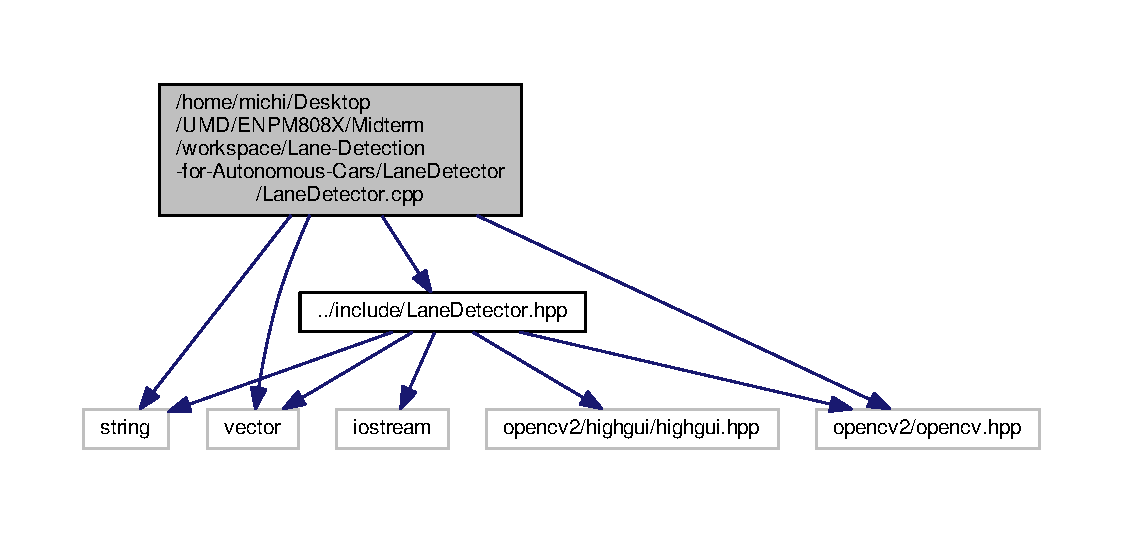
\includegraphics[width=350pt]{LaneDetector_8cpp__incl}
\end{center}
\end{figure}
This graph shows which files directly or indirectly include this file\+:
\nopagebreak
\begin{figure}[H]
\begin{center}
\leavevmode
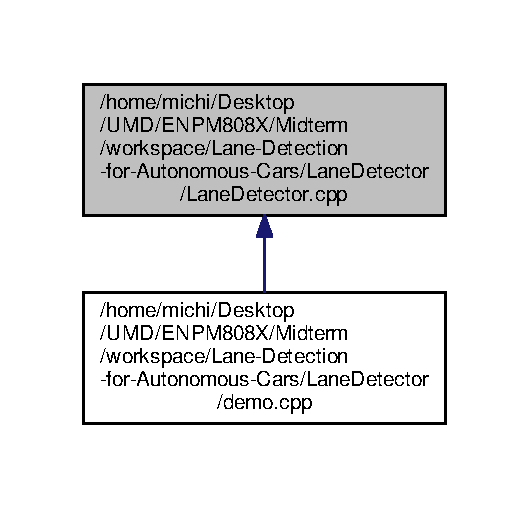
\includegraphics[width=254pt]{LaneDetector_8cpp__dep__incl}
\end{center}
\end{figure}


\subsection{Detailed Description}
Definition of all the function that form part of the \hyperlink{classLaneDetector}{Lane\+Detector} class. 

M\+IT License Copyright (c) 2017 Miguel Maestre Trueba Permission is hereby granted, free of charge, to any person obtaining a copy of this software and associated documentation files (the \char`\"{}\+Software\char`\"{}), to deal in the Software without restriction, including without limitation the rights to use, copy, modify, merge, publish, distribute, sublicense, and/or sell copies of the Software, and to permit persons to whom the Software is furnished to do so, subject to the following conditions\+: The above copyright notice and this permission notice shall be included in all copies or substantial portions of the Software. T\+HE S\+O\+F\+T\+W\+A\+RE IS P\+R\+O\+V\+I\+D\+ED \char`\"{}\+A\+S I\+S\char`\"{}, W\+I\+T\+H\+O\+UT W\+A\+R\+R\+A\+N\+TY OF A\+NY K\+I\+ND, E\+X\+P\+R\+E\+SS OR I\+M\+P\+L\+I\+ED, I\+N\+C\+L\+U\+D\+I\+NG B\+UT N\+OT L\+I\+M\+I\+T\+ED TO T\+HE W\+A\+R\+R\+A\+N\+T\+I\+ES OF M\+E\+R\+C\+H\+A\+N\+T\+A\+B\+I\+L\+I\+TY, F\+I\+T\+N\+E\+SS F\+OR A P\+A\+R\+T\+I\+C\+U\+L\+AR P\+U\+R\+P\+O\+SE A\+ND N\+O\+N\+I\+N\+F\+R\+I\+N\+G\+E\+M\+E\+NT. IN NO E\+V\+E\+NT S\+H\+A\+LL T\+HE A\+U\+T\+H\+O\+RS OR C\+O\+P\+Y\+R\+I\+G\+HT H\+O\+L\+D\+E\+RS BE L\+I\+A\+B\+LE F\+OR A\+NY C\+L\+A\+IM, D\+A\+M\+A\+G\+ES OR O\+T\+H\+ER L\+I\+A\+B\+I\+L\+I\+TY, W\+H\+E\+T\+H\+ER IN AN A\+C\+T\+I\+ON OF C\+O\+N\+T\+R\+A\+CT, T\+O\+RT OR O\+T\+H\+E\+R\+W\+I\+SE, A\+R\+I\+S\+I\+NG F\+R\+OM, O\+UT OF OR IN C\+O\+N\+N\+E\+C\+T\+I\+ON W\+I\+TH T\+HE S\+O\+F\+T\+W\+A\+RE OR T\+HE U\+SE OR O\+T\+H\+ER D\+E\+A\+L\+I\+N\+GS IN T\+HE S\+O\+F\+T\+W\+A\+RE.

\begin{DoxyCopyright}{Copyright}
Copyright 2017 Miguel Maestre Trueba
\end{DoxyCopyright}
\begin{DoxyAuthor}{Author}
Miguel Maestre Trueba The class will take R\+GB images as inputs and will output the same R\+GB image but with the plot of the detected lanes and the turn prediction. 
\end{DoxyAuthor}

\hypertarget{main_8cpp}{}\section{/home/michi/\+Desktop/\+U\+M\+D/\+E\+N\+P\+M808\+X/\+Midterm/workspace/\+Lane-\/\+Detection-\/for-\/\+Autonomous-\/\+Cars/test/main.cpp File Reference}
\label{main_8cpp}\index{/home/michi/\+Desktop/\+U\+M\+D/\+E\+N\+P\+M808\+X/\+Midterm/workspace/\+Lane-\/\+Detection-\/for-\/\+Autonomous-\/\+Cars/test/main.\+cpp@{/home/michi/\+Desktop/\+U\+M\+D/\+E\+N\+P\+M808\+X/\+Midterm/workspace/\+Lane-\/\+Detection-\/for-\/\+Autonomous-\/\+Cars/test/main.\+cpp}}


Test cases for code coverage.  


{\ttfamily \#include $<$gtest/gtest.\+h$>$}\\*
Include dependency graph for main.\+cpp\+:
\nopagebreak
\begin{figure}[H]
\begin{center}
\leavevmode
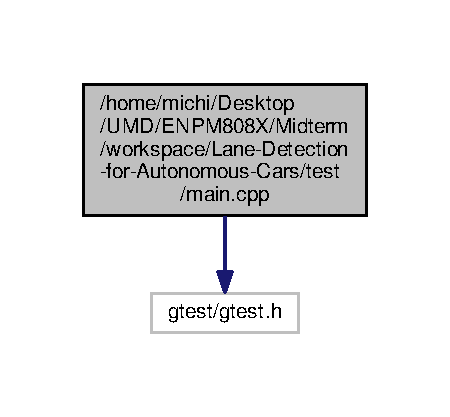
\includegraphics[width=216pt]{main_8cpp__incl}
\end{center}
\end{figure}
\subsection*{Functions}
\begin{DoxyCompactItemize}
\item 
int {\bfseries main} (int argc, char $\ast$$\ast$argv)\hypertarget{main_8cpp_a3c04138a5bfe5d72780bb7e82a18e627}{}\label{main_8cpp_a3c04138a5bfe5d72780bb7e82a18e627}

\end{DoxyCompactItemize}


\subsection{Detailed Description}
Test cases for code coverage. 

M\+IT License Copyright (c) 2017 Miguel Maestre Trueba Permission is hereby granted, free of charge, to any person obtaining a copy of this software and associated documentation files (the \char`\"{}\+Software\char`\"{}), to deal in the Software without restriction, including without limitation the rights to use, copy, modify, merge, publish, distribute, sublicense, and/or sell copies of the Software, and to permit persons to whom the Software is furnished to do so, subject to the following conditions\+: The above copyright notice and this permission notice shall be included in all copies or substantial portions of the Software. T\+HE S\+O\+F\+T\+W\+A\+RE IS P\+R\+O\+V\+I\+D\+ED \char`\"{}\+A\+S I\+S\char`\"{}, W\+I\+T\+H\+O\+UT W\+A\+R\+R\+A\+N\+TY OF A\+NY K\+I\+ND, E\+X\+P\+R\+E\+SS OR I\+M\+P\+L\+I\+ED, I\+N\+C\+L\+U\+D\+I\+NG B\+UT N\+OT L\+I\+M\+I\+T\+ED TO T\+HE W\+A\+R\+R\+A\+N\+T\+I\+ES OF M\+E\+R\+C\+H\+A\+N\+T\+A\+B\+I\+L\+I\+TY, F\+I\+T\+N\+E\+SS F\+OR A P\+A\+R\+T\+I\+C\+U\+L\+AR P\+U\+R\+P\+O\+SE A\+ND N\+O\+N\+I\+N\+F\+R\+I\+N\+G\+E\+M\+E\+NT. IN NO E\+V\+E\+NT S\+H\+A\+LL T\+HE A\+U\+T\+H\+O\+RS OR C\+O\+P\+Y\+R\+I\+G\+HT H\+O\+L\+D\+E\+RS BE L\+I\+A\+B\+LE F\+OR A\+NY C\+L\+A\+IM, D\+A\+M\+A\+G\+ES OR O\+T\+H\+ER L\+I\+A\+B\+I\+L\+I\+TY, W\+H\+E\+T\+H\+ER IN AN A\+C\+T\+I\+ON OF C\+O\+N\+T\+R\+A\+CT, T\+O\+RT OR O\+T\+H\+E\+R\+W\+I\+SE, A\+R\+I\+S\+I\+NG F\+R\+OM, O\+UT OF OR IN C\+O\+N\+N\+E\+C\+T\+I\+ON W\+I\+TH T\+HE S\+O\+F\+T\+W\+A\+RE OR T\+HE U\+SE OR O\+T\+H\+ER D\+E\+A\+L\+I\+N\+GS IN T\+HE S\+O\+F\+T\+W\+A\+RE.

\begin{DoxyCopyright}{Copyright}
Copyright 2017 Miguel Maestre Trueba
\end{DoxyCopyright}
\begin{DoxyAuthor}{Author}
Miguel Maestre Trueba 
\end{DoxyAuthor}

\hypertarget{test_8cpp}{}\section{/home/michi/\+Desktop/\+U\+M\+D/\+E\+N\+P\+M808\+X/\+Midterm/workspace/\+Lane-\/\+Detection-\/for-\/\+Autonomous-\/\+Cars/test/test.cpp File Reference}
\label{test_8cpp}\index{/home/michi/\+Desktop/\+U\+M\+D/\+E\+N\+P\+M808\+X/\+Midterm/workspace/\+Lane-\/\+Detection-\/for-\/\+Autonomous-\/\+Cars/test/test.\+cpp@{/home/michi/\+Desktop/\+U\+M\+D/\+E\+N\+P\+M808\+X/\+Midterm/workspace/\+Lane-\/\+Detection-\/for-\/\+Autonomous-\/\+Cars/test/test.\+cpp}}


Test cases for code coverage.  


{\ttfamily \#include $<$opencv2/highgui/highgui.\+hpp$>$}\\*
{\ttfamily \#include $<$gtest/gtest.\+h$>$}\\*
{\ttfamily \#include $<$iostream$>$}\\*
{\ttfamily \#include $<$string$>$}\\*
{\ttfamily \#include $<$vector$>$}\\*
{\ttfamily \#include \char`\"{}opencv2/opencv.\+hpp\char`\"{}}\\*
{\ttfamily \#include \char`\"{}../include/\+Lane\+Detector.\+hpp\char`\"{}}\\*
Include dependency graph for test.\+cpp\+:
\nopagebreak
\begin{figure}[H]
\begin{center}
\leavevmode
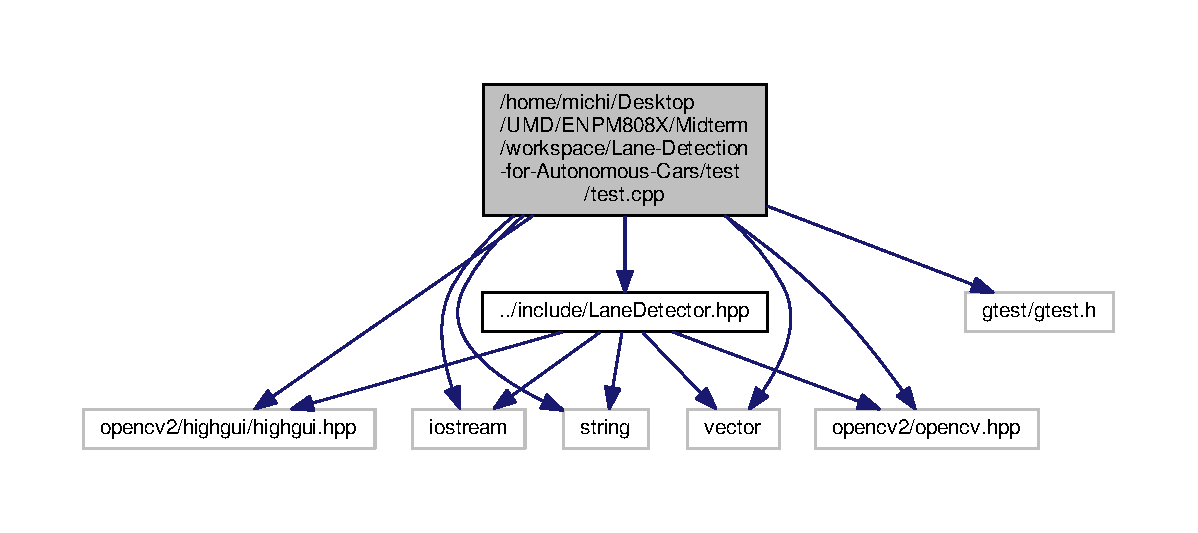
\includegraphics[width=350pt]{test_8cpp__incl}
\end{center}
\end{figure}
\subsection*{Functions}
\begin{DoxyCompactItemize}
\item 
int \hyperlink{test_8cpp_a8189074c445602673a444b132ef6b71e}{testing\+\_\+lanes} (int video, int frame\+\_\+number)
\begin{DoxyCompactList}\small\item\em Function very similar to \hyperlink{demo_8cpp}{demo.\+cpp}. It tests only one iteration of the algorithm for a single image. \end{DoxyCompactList}\item 
\hyperlink{test_8cpp_ad71fa10af78b3c1d7a6ff06e6d1ce111}{T\+E\+ST} (Lane\+Test, lane\+\_\+detected)\hypertarget{test_8cpp_ad71fa10af78b3c1d7a6ff06e6d1ce111}{}\label{test_8cpp_ad71fa10af78b3c1d7a6ff06e6d1ce111}

\begin{DoxyCompactList}\small\item\em Test case to test if lane is detected and if the lane is turning left. \end{DoxyCompactList}\item 
\hyperlink{test_8cpp_ad6f42a29b11367b38cd4c5495ff2d751}{T\+E\+ST} (Lane\+Test, no\+\_\+turn)\hypertarget{test_8cpp_ad6f42a29b11367b38cd4c5495ff2d751}{}\label{test_8cpp_ad6f42a29b11367b38cd4c5495ff2d751}

\begin{DoxyCompactList}\small\item\em Test cases to test if lane is detected and if the lane is going straight. \end{DoxyCompactList}\item 
\hyperlink{test_8cpp_a8561acb13779f6ced5a6775d94f08438}{T\+E\+ST} (Lane\+Test, right\+\_\+turn)\hypertarget{test_8cpp_a8561acb13779f6ced5a6775d94f08438}{}\label{test_8cpp_a8561acb13779f6ced5a6775d94f08438}

\begin{DoxyCompactList}\small\item\em Test cases to test if lane is detected and if the lane is turning right. \end{DoxyCompactList}\item 
\hyperlink{test_8cpp_a8506b1e97f3c8065cc61e3977197a70d}{T\+E\+ST} (Lane\+Test, lane\+\_\+not\+\_\+detected)\hypertarget{test_8cpp_a8506b1e97f3c8065cc61e3977197a70d}{}\label{test_8cpp_a8506b1e97f3c8065cc61e3977197a70d}

\begin{DoxyCompactList}\small\item\em Test cases to test if lane is not detected at all. \end{DoxyCompactList}\end{DoxyCompactItemize}


\subsection{Detailed Description}
Test cases for code coverage. 

M\+IT License Copyright (c) 2017 Miguel Maestre Trueba Permission is hereby granted, free of charge, to any person obtaining a copy of this software and associated documentation files (the \char`\"{}\+Software\char`\"{}), to deal in the Software without restriction, including without limitation the rights to use, copy, modify, merge, publish, distribute, sublicense, and/or sell copies of the Software, and to permit persons to whom the Software is furnished to do so, subject to the following conditions\+: The above copyright notice and this permission notice shall be included in all copies or substantial portions of the Software. T\+HE S\+O\+F\+T\+W\+A\+RE IS P\+R\+O\+V\+I\+D\+ED \char`\"{}\+A\+S I\+S\char`\"{}, W\+I\+T\+H\+O\+UT W\+A\+R\+R\+A\+N\+TY OF A\+NY K\+I\+ND, E\+X\+P\+R\+E\+SS OR I\+M\+P\+L\+I\+ED, I\+N\+C\+L\+U\+D\+I\+NG B\+UT N\+OT L\+I\+M\+I\+T\+ED TO T\+HE W\+A\+R\+R\+A\+N\+T\+I\+ES OF M\+E\+R\+C\+H\+A\+N\+T\+A\+B\+I\+L\+I\+TY, F\+I\+T\+N\+E\+SS F\+OR A P\+A\+R\+T\+I\+C\+U\+L\+AR P\+U\+R\+P\+O\+SE A\+ND N\+O\+N\+I\+N\+F\+R\+I\+N\+G\+E\+M\+E\+NT. IN NO E\+V\+E\+NT S\+H\+A\+LL T\+HE A\+U\+T\+H\+O\+RS OR C\+O\+P\+Y\+R\+I\+G\+HT H\+O\+L\+D\+E\+RS BE L\+I\+A\+B\+LE F\+OR A\+NY C\+L\+A\+IM, D\+A\+M\+A\+G\+ES OR O\+T\+H\+ER L\+I\+A\+B\+I\+L\+I\+TY, W\+H\+E\+T\+H\+ER IN AN A\+C\+T\+I\+ON OF C\+O\+N\+T\+R\+A\+CT, T\+O\+RT OR O\+T\+H\+E\+R\+W\+I\+SE, A\+R\+I\+S\+I\+NG F\+R\+OM, O\+UT OF OR IN C\+O\+N\+N\+E\+C\+T\+I\+ON W\+I\+TH T\+HE S\+O\+F\+T\+W\+A\+RE OR T\+HE U\+SE OR O\+T\+H\+ER D\+E\+A\+L\+I\+N\+GS IN T\+HE S\+O\+F\+T\+W\+A\+RE.

\begin{DoxyCopyright}{Copyright}
Copyright 2017 Miguel Maestre Trueba
\end{DoxyCopyright}
\begin{DoxyAuthor}{Author}
Miguel Maestre Trueba 
\end{DoxyAuthor}


\subsection{Function Documentation}
\index{test.\+cpp@{test.\+cpp}!testing\+\_\+lanes@{testing\+\_\+lanes}}
\index{testing\+\_\+lanes@{testing\+\_\+lanes}!test.\+cpp@{test.\+cpp}}
\subsubsection[{\texorpdfstring{testing\+\_\+lanes(int video, int frame\+\_\+number)}{testing_lanes(int video, int frame_number)}}]{\setlength{\rightskip}{0pt plus 5cm}int testing\+\_\+lanes (
\begin{DoxyParamCaption}
\item[{int}]{video, }
\item[{int}]{frame\+\_\+number}
\end{DoxyParamCaption}
)}\hypertarget{test_8cpp_a8189074c445602673a444b132ef6b71e}{}\label{test_8cpp_a8189074c445602673a444b132ef6b71e}


Function very similar to \hyperlink{demo_8cpp}{demo.\+cpp}. It tests only one iteration of the algorithm for a single image. 


\begin{DoxyParams}{Parameters}
{\em video} & is a flag that selects the demo video or an image without lanes for testing purposes \\
\hline
{\em frame\+\_\+number} & gives the exact frame number of the input video \\
\hline
\end{DoxyParams}
\begin{DoxyReturn}{Returns}
flag\+\_\+plot tells if the demo has sucessfully finished 
\end{DoxyReturn}

%--- End generated contents ---

% Index
\backmatter
\newpage
\phantomsection
\clearemptydoublepage
\addcontentsline{toc}{chapter}{Index}
\printindex

\end{document}
